\section*{Dioptra}

\item 
\begin{enumerate}
	\item (*) Demostrar que un haz homocéntrico de pequeña abertura que incide casi normal sobre una dioptra plana, da lugar a otro haz homocéntrico.
	Considere los casos de objetos reales y virtuales.
	\item Una moneda se encuentra en el fondo de un vaso que contiene agua hasta una altura de 5 cm ($n_{agua}=1.33$).
	Un observador la mira desde arriba, ¿a qué profundidad la ve?
	\item (*) Estimar la máxima abertura de un haz homocéntrico, para que la posición de la imagen, formada por una única superficie plana, quede determinada con un error del 2\%. 
\end{enumerate}


\item (*) Usando los resultados del problema anterior demuestre que un haz homocéntrico de pequeña abertura, al atravesar una lámina de caras paralelas, da lugar, en primera aproximación, a otro haz homocéntrico.
Halle la posición de las sucesivas imágenes. 


\item
\begin{minipage}[t][1.4cm]{0.55\textwidth}
	Analice la figura con la ley de Ibn Sahl - Snell haciendo uso de la aproximación paraxial $\alpha \approx \sen( \alpha ) \approx \tan( \alpha )$ (lo mismo pasa con $\beta$ y $\varphi$) 
\end{minipage}
\begin{minipage}[c][0.4cm][t]{0.4\textwidth}
	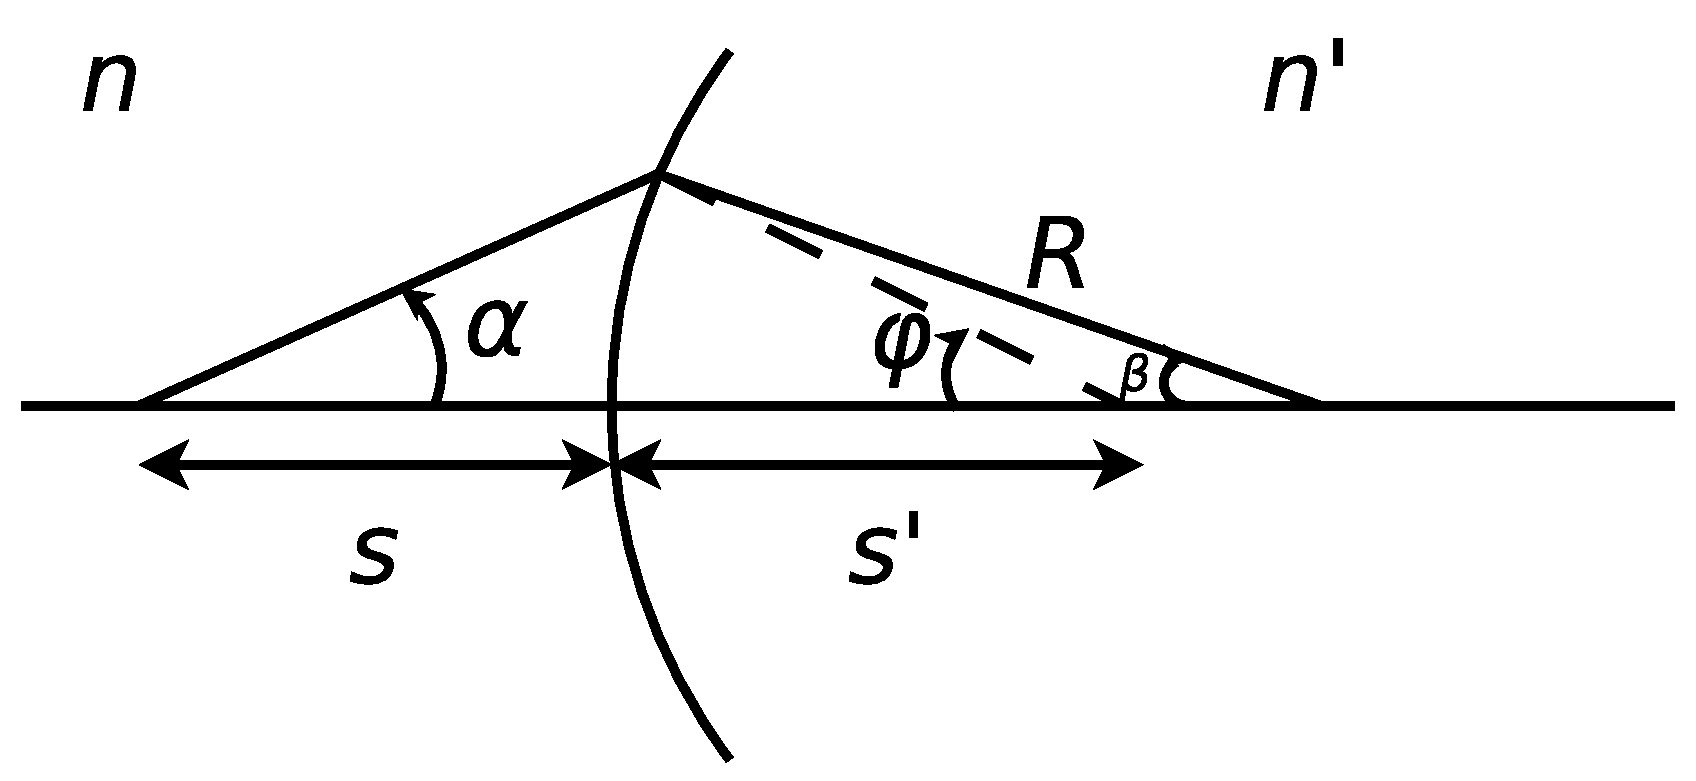
\includegraphics[width=\textwidth]{ej3-15}
\end{minipage}
\begin{enumerate}
	\item
	Obtenga la ecuación de las dioptras esféricas
	\[
		\frac{n'}{s'}\mp\frac{n}{s}=\frac{(n'-n)}{R} .
	\]
	Discuta el doble signo, asociándolo con la convención de signos que se utilice.
	\item Para una dioptra esférica arbitraria haga un gráfico $s'$ vs. $s$ y analice a partir de él para qué posiciones de los objetos reales las imágenes son reales o virtuales, directas o invertidas y lo mismo para objetos virtuales.
	Analice todos los casos posibles para dioptras convergentes y divergentes.
	\item ¿Pueden ser iguales las dos distancias focales de una dioptra?
	Justifique su respuesta.
\end{enumerate}

